%%This is a very basic article template.
%%There is just one section and two subsections.
\documentclass{article}

\usepackage[style=numeric,backend=bibtex]{biblatex}
\usepackage{graphicx}
\usepackage{tabulary}
\usepackage{hyperref}

\bibliography{bib}

\begin{document}


\section*{Dynamic Perfect Hashing - Implementation}

by Lennart Hensler and Frederik Petersen

\section{Introduction}

Dynamic perfect hashing allows for constant find and amortized constant inserts.
We implemented a variant based on \cite{di94}, which uses a two layer approach
to avoid the need of $ n^2 $ space. The outer layer consists of a number of
buckets with a hash function that distributes the data into the buckets. There
may be collisions. Each bucket has its own inner hash function and allows
perfect hashing. If perfect hashing can not be provided in a bucket the data
structure can be resized and/or new hash functions are generated depending on
some conditions. It can also be necessary to completely rehash the table. \cite{di94} describes two reasons to do this.
\begin{enumerate}
  \item A counter of the hash table is greater or equals to a threshold.
  \begin{itemize}
    \item The counter is increased when a new key is inserted in the table and when an entry is deleted.
    \item The threshold depends on the amount of entries that are contained by the table.
  \end{itemize}
  \item A global condition isn't satisfied after a bucket has been resized.
\end{enumerate}

\section {Approaches}

We implemented three different approaches for the dynamic perfect hashing. The first two stick close to \cite{di94}, but have different data structures. The third tries to solve the problem with less mathematic, but in a more pragmatical way. The implementation of these approaches is available on github\footnote{\href{https://github.com/FrederikP/algen-framework}{https://github.com/FrederikP/algen-framework}}.

\subsection{Storing all entries in a single vector}

At first we tried to store all the entries in one single array instead of using multiple buckets as described in \cite[p. 94]{mesa08}. The buckets are represented with meta information like the index of the start of the bucket, the bucket length and its hash function. We had a lot of issues due to the immense copying/moving needed, when resizing one of the buckets. This could be avoided when giving all the buckets some extra space in the array, which they can grow into without the need to touch other buckets. This, again, would increase the space requirements. This approach is in the file \texttt{DPH\_with\_single\_vector.h}.

\subsection{Storing the entries in buckets}

In this case every bucket stores the data in its own vector and the table consists of a vector of buckets. This approach is much more efficient than the simple approach with a single vector. We implemented this approach in two different ways. The first sticks close to \cite{di94} (rehashing logic, counters for the table and the buckets) and is in the file \texttt{DPH\_with\_buckets.h}. The second one tries to solve the problem in a more pragmatic way. We removed the counters and the thresholds and the resizing/rehashing is now based on the amount of elements contained by the table/bucket and its capacity. This approach is in the file \texttt{DPH\_with\_buckets\_2.h}. We isolated six parameters, that affect the performance and the needed space for the approaches with buckets.

\section{Parameters}

Several parameters have an impact on the performance and needed space of the
algorithm. We will have a look at several parameters here.

\begin{itemize}
  \item \textbf{Bucket Capacity Factor}\\
  	How much bigger than the number of current elements will a bucket be created for (capacity-wise). In the approach with counters and thresholds is the threshold of a bucket equal to its capacity.
  \item \textbf{Bucket Length Factor}\\
    How much bigger than the desired capacity will a bucket be. The smaller this is, the faster the data structure needs to be updated. The larger it is, the more space is needed per element.
  \item \textbf{Maximum Number of Rehash Attempts}\\
  	How often can the guessing of a new injective hash function of a bucket fail, before the bucket gets resized. The smaller it is, the faster is the rehashing. But if this value is to small, it's possible that the bucket becomes bigger than necessary.
  \item \textbf{Rehash Length Factor}\\
    The factor the bucket length will be multiplied with, if the maximum number of rehash attempts is exceeded. The bigger it is, the unlikely it's necessary to resize the bucket again. But if this value is to big, the bucket will become bigger than necessary.
  \item \textbf{Table Capacity Factor}\\
    In the approach with counters and thresholds affects this parameter the threshold of the table: $ threshold = (1 + factor) * \max(elementAmount, 4) $
    In the pragmatic approach affects is the capacity of the table equal to the number of contained elements multiplied with the factor.
  \item \textbf{Element Amount per Bucket}\\
    The starting capacity of the buckets after the table has been initialized or rehashed. The bigger it is, the less buckets will be created.
\end{itemize}

After some experimenting with these parameters, the following values seem to create the best results.

\begin{center}
\begin{tabulary}{0.95\textwidth}{R|C|C}
& With counters \newline and thresholds & Pragmatic approach \\ 
\hline Bucket Capacity Factor & 7 & 2 \\ 
\hline Bucket Length Factor & 2 & 2 \\ 
\hline Maximum Number of Rehash Attempts & 5 & 5 \\ 
\hline Rehash Length Factor & 2 & 2 \\ 
\hline Table Capacity Factor & 6 & 2 \\ 
\hline Element Amount per Bucket & 3500 & 3000 \\
\end{tabulary}
\end{center}

\section{Experiment Results}

We ran our experiments on a quad core Intel Atom server running a 32bit Debian
Jessie OS with 4GB of RAM. The benchmarks were run automatically each time a
code update was pushed to the repository and plots were generated and saved per
build. That allowed us to test different parameters and compare them to the
earlier builds.\\

\centering
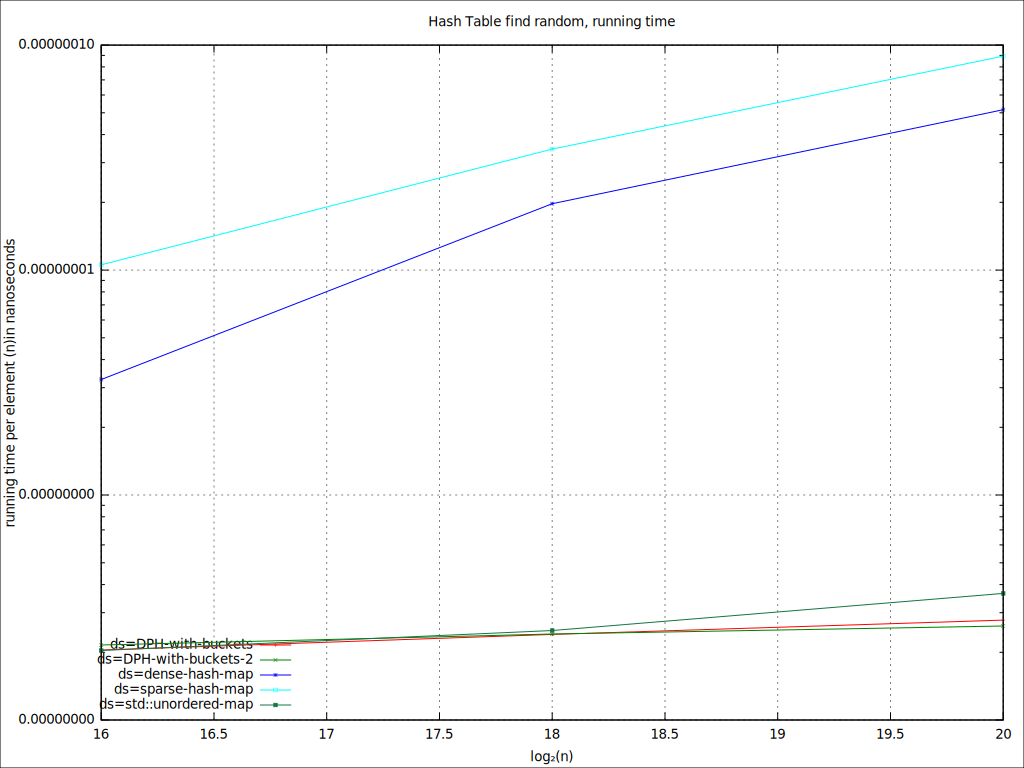
\includegraphics[width=0.9\linewidth]{img/hash_find-random_time}

\printbibliography

\end{document}
